\documentclass[convert]{standalone}

\usepackage{tikz}
\usepackage{graphicx}
\pagestyle{empty}

% INT_AY22_L28-Fig01_Ampere_circuit.png

\begin{document}
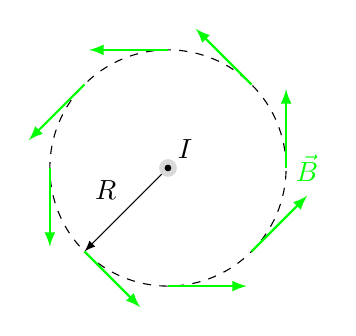
\begin{tikzpicture}[> = latex]

	% Definition
	
	\def\R{1.5}		% Size of amperian path
	
	% Radius indicator
	
	\draw [->] (0, 0) -- node [above left] {$R$} (225 : \R);

	% Wire w/ current
	
	\filldraw [gray!30] (0, 0) circle (3 pt) node [black, above right] {$I$};
	\filldraw (0, 0) circle (1 pt);
	
	% Amperian path
	
	\draw [dashed] (0, 0) circle (\R cm);
	
	% Magnetic field vectors on path
	
	\foreach \Q in {0, 45, ..., 315}
		\draw [thick, green, ->] (\Q : \R) -- ++ ({\Q + 90} : 1);
		
	\node [right, green] at (\R, 0) {${\vec B}$};

\end{tikzpicture}
\end{document}